\chapter{Aplicación}

\chapter{Capa de Aplicación}

\section{Introducción}
En esta capa de aplicaciones observaremos los principales conceptos de comunicación entre componentes por medio de interfaces, donde en los siguientes diagramas se pueden observar los principales comportamientos del aplicativo mediante 4 puntos de vista: Comportamiento de aplicación, Cooperación de aplicación, Estructura de aplicación y el uso de la aplicación.\\
Tal como mencionamos anteriormente, en nuestra capa de aplicación se caracteriza por poseer una arquitectura de componentes, de tal forma que  mostramos las principales funciones dentro de cada componente y ademas como se relacionan y comunican cada uno de estos, de tal forma que observemos como sera el comportamiento y la logica de la aplicación

\section{Punto de Vista de Comportamiento de Aplicación}
\subsection{Descripción}
El punto de vista de comportamiento de aplicación, describe el comportamiento interno de la aplicación, que este realiza uno o más servicios de aplicaciones. El punto de vista es útil en diseñar el principal comportamiento de la aplicación, o identificar superposición funcional entre diferentes aplicación.

\subsubsection{Metamodelo}
\begin{figure}[H]
	\centering
	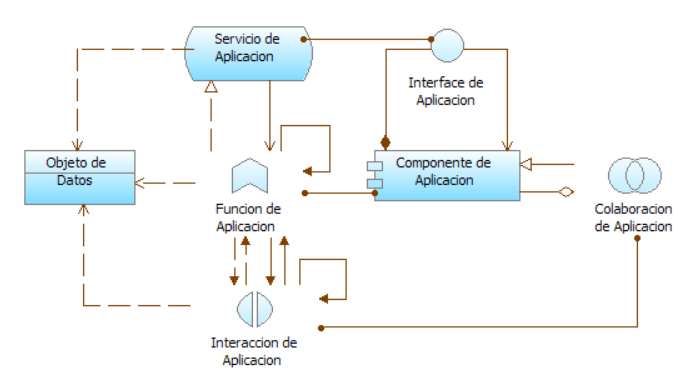
\includegraphics[width=1.0\textwidth]{imagenes/Metamodelos/Aplicacion/meta_comportamiento_aplicacion.png}
	\caption{Metamodelo: Punto de Vista de Comportamiento de Aplicación.}
	\label{fig:gap_analysis}
\end{figure}

\subsubsection{Caso de Estudio}
En el presente caso de estudio, podemos observar el componente aplicación de la aplicación Two Wheels Digital, el cual se divide compone a su vez de componentes más pequeños como lo son Pagos, que se encarga de cumplir las funciones de cálculo de la tarifa y recepción del pago realizado por cada cliente. Por otra parte, el Gestor de Espacios encargado de la administración de los espacios de parqueo; el Gestor de Usuarios quien lleva a cabo el proceso de registro y validación. Por último, el componente de Estadísticas el cual elabora reportes sobre la renta de los espacios de parqueo.
\begin{figure}[H]
	\centering
	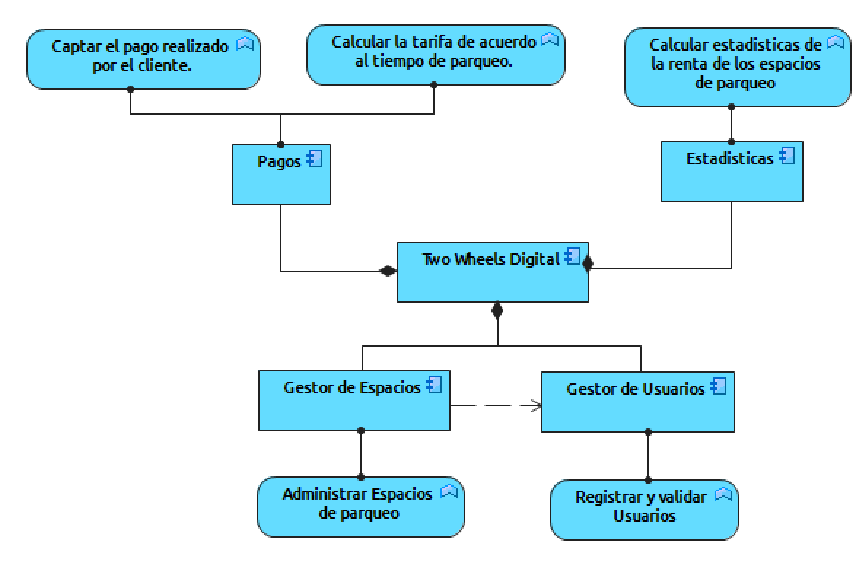
\includegraphics[width=1.0\textwidth]{imagenes/Caso_Estudio/Aplicacion/ComAplicacion.PDF}
	\caption{Caso de estudio: Punto de vista de comportamiento de aplicación.}
	\label{fig:gap_analysis}
\end{figure}




\section{Punto de Vista de Cooperación de Aplicación}
\subsection{Descripción}
El punto de vista Cooperación de aplicación describe las relaciones entre los componentes de la aplicaciones en términos de la información que se maneja entre ellos además de esto también se puede enfocar en términos de los servicios que estos ofrecen y de los que hacen uso. Este punto de vista también es usado para crear una visión general de todo el contexto de aplicación de una organización. Este punto de vista también es usado para expresar la cooperación interna de servicios que trabajando de una forma conjunta soportan la ejecución de un proceso de negocio.

\subsubsection{Metamodelo}
\begin{figure}[H]
	\centering
	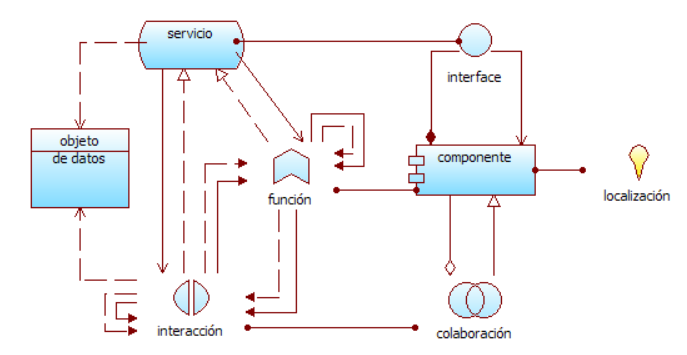
\includegraphics[width=1.0\textwidth]{imagenes/Metamodelos/Aplicacion/meta_cooperacion_aplicacion.png}
	\caption{Metamodelo: Punto de Vista de Cooperación de Aplicación.}
	\label{fig:gap_analysis}
\end{figure}

\subsubsection{Caso de Estudio}
Por medio de este punto de vista, se resalta la arquitectura general de tres capas de la aplicación Two Wheels Digital en donde el componente principal de interfaz se encuentra ubicado en la capa de presentación; los componentes Gestor de Usuarios, Gestor de Espacios, Pagos y Estadísticas se ubican en la capa de negocio, y finalmente el componente de almacenamiento, Base de Datos, se ubica en la capa de persistencia.

\begin{figure}[H]
	\centering
	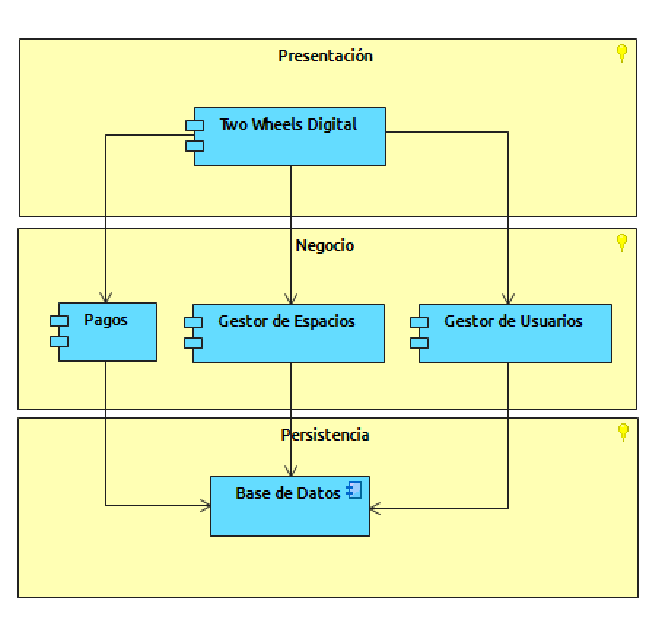
\includegraphics[width=1.0\textwidth]{imagenes/Caso_Estudio/Aplicacion/CoopAplicacion.PDF}
	\caption{Caso de estudio: Punto de vista de cooperación de aplicación.}
	\label{fig:gap_analysis}
\end{figure}






\section{Punto de Vista de Uso de Aplicación}
\subsection{Descripción}
El punto de vista Uso de aplicaciones describe cómo se utilizan las aplicaciones para soportar uno o más procesos empresariales y cómo se utilizan en otras aplicaciones. Se puede utilizar en el diseño de una aplicación mediante la identificación de los servicios necesarios por los procesos de negocio y otras aplicaciones, o en el diseño de procesos de negocio mediante la descripción de los servicios que están disponibles. Además, puesto que identifica las dependencias de los procesos de negocio en las aplicaciones, puede ser útil para los gerentes operacionales responsables de estos procesos.

\subsubsection{Metamodelo}
\begin{figure}[H]
	\centering
	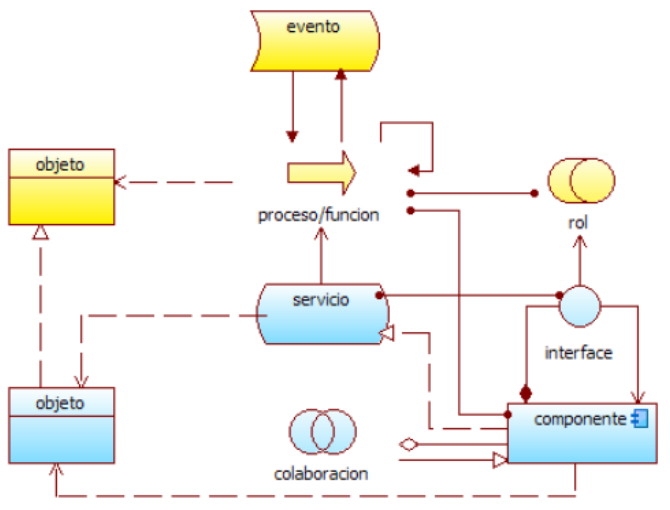
\includegraphics[width=1.0\textwidth]{imagenes/Metamodelos/Aplicacion/meta_uso_aplicacion.png}
	\caption{Metamodelo: Punto de Vista de Uso de Aplicación.}
	\label{fig:gap_analysis}
\end{figure}

\subsubsection{Caso de Estudio}
Se tiene como enfoque principal el proceso de Renta de espacios de parqueadero el cual hace uso de tres servicios llevados a cabo por el componente principal de la aplicación Two Wheels Digital, como lo son la gestión de usuarios, la gestión de espacios y la gestión de pagos.

\begin{figure}[H]
	\centering
	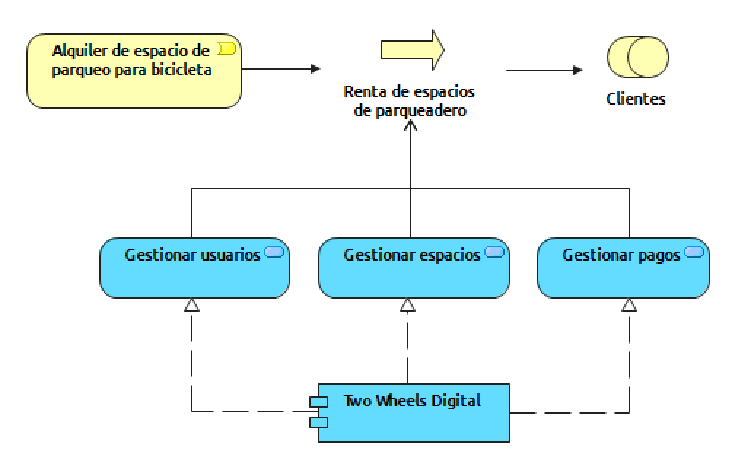
\includegraphics[width=1.0\textwidth]{imagenes/Caso_Estudio/Aplicacion/UsoAplicacion.PDF}
	\caption{Caso de estudio: Punto de vista de Uso de aplicación.}
	\label{fig:gap_analysis}
\end{figure}

\section{Punto de vista de Estructura de Aplicación}
\subsection{Descripción}
El punto de vista de Estructura de la aplicación muestra la estructura de una o más aplicaciones
o componentes. Este punto de vista es útil para diseñar o comprender la estructura principal de
aplicaciones o componentes y los datos asociados, por ejemplo, para descomponer la estructura del
sistema en construcción o para identificar componentes de aplicación heredados que son adecuados
para la migración/integración.

\subsubsection{Metamodelo}
\begin{figure}[H]
	\centering
	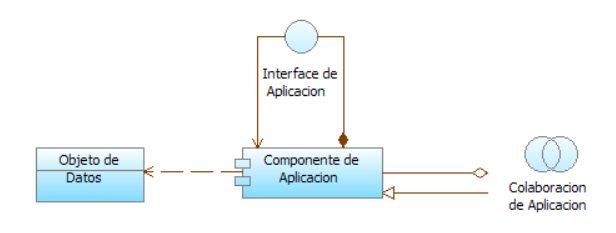
\includegraphics[width=1.0\textwidth]{imagenes/Metamodelos/Aplicacion/meta_estructura_aplicacion.png}
	\caption{Metamodelo: Punto de Vista de Estructura de Aplicación.}
	\label{fig:gap_analysis}
\end{figure}

\subsubsection{Caso de Estudio}

\begin{figure}[H]
	\centering
	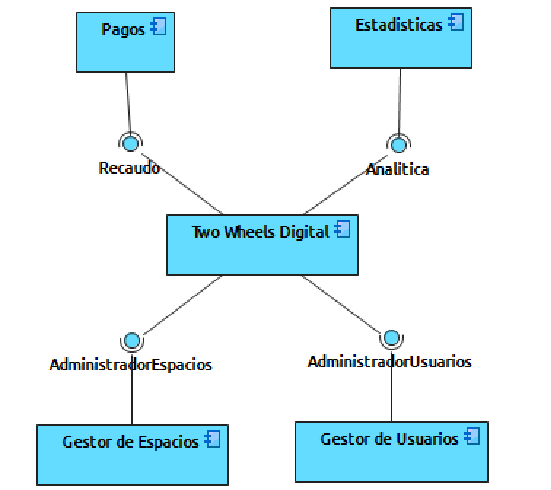
\includegraphics[width=1.0\textwidth]{imagenes/Caso_Estudio/Aplicacion/EstAplicacion.PDF}
	\caption{Caso de estudio: Punto de vista de estructura de aplicación.}
	\label{fig:gap_analysis}
\end{figure}
